\documentclass[a4paper,12pt]{report} % Format du papier, type de document
 
\usepackage[utf8]{inputenc} % Permet de tapper les accents tels quels
\usepackage[T1]{fontenc} % Permet l'utilisation d'accents
\usepackage[french]{babel} % Dit que le document est en français
\usepackage{amsfonts} % Différents packages... Lire la doc....
\usepackage{amsmath}
\usepackage{listings}
\usepackage{color}
\usepackage{graphicx} %affichage d'image
\usepackage{moreverb}
\usepackage[colorlinks=true,linkcolor=black]{hyperref} %lien hypertexte
\usepackage{fullpage}
\usepackage{fancyhdr}
\pagestyle{fancy}
\renewcommand{\thesection}{\arabic{section}}
\setcounter{tocdepth}{5}
\setcounter{secnumdepth}{5}

\renewcommand{\headrulewidth}{0pt} 
\fancyhead{} %retire en tete

\renewcommand{\footrulewidth}{1pt} %bas de page
\fancyfoot[C]{} 
\fancyfoot[L]{Rapport réseau \textbf{\thepage}}
\fancyfoot[R]{DUCRUET Corentin - Gheysen Jérémy}

\title{Projet de réseau II\\Rapport}
\author{UMONS\\Faculté des Sciences\\MA 1 Sciences - Informatique\\DUCRUET Corentin \\Gheysen Jérémy}}
\date{Année académique\\2016 - 2017}





%\begin{figure}[!h] %on ouvre l'environnement figure
%		\centering
%		\includegraphics[width=108mm,height=65mm]{impulsion.png}
%	\end{figure} 

%\begin{figure}%[H] si on veut que l image soit a cet endroit
%	\centering
%	\includegraphics[width=108mm,height=65mm]{./scr/logo}
%	\caption{Icône}
%	\label{fig:Icône}
%\end{figure}

\begin{document} 
\maketitle
\newpage 
\tableofcontents 
\newpage
\raggedright

\section{Introduction}
Le but de ce projet était de modéliser une interconnexion de réseau en utilisant C-BGP. Il nous était demander de réaliser une configuration complète de plusieurs routeurs appartenant à divers domaines.

\section{Choix de design}
La topologie que nous devions implémenter était la suivante:
\begin{figure}[!h] %on ouvre l'environnement figure
		\centering
		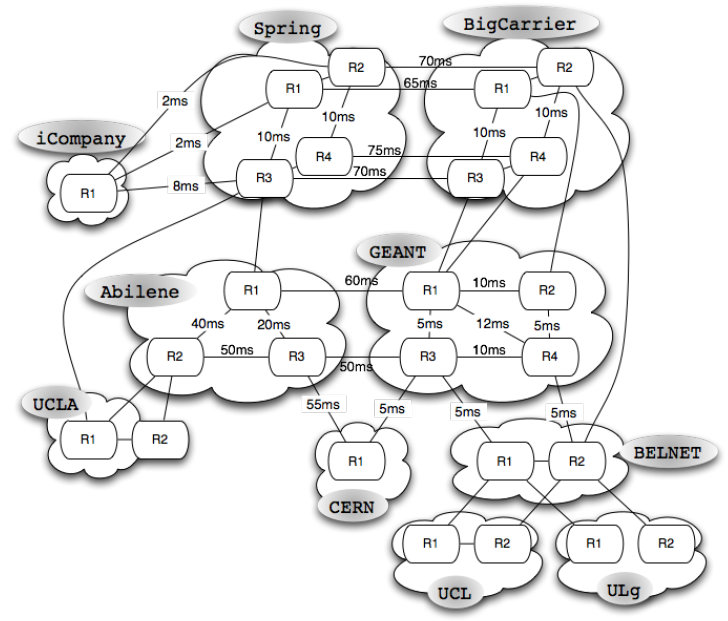
\includegraphics[width=120mm,height=80mm]{topologie}
		\label{topo}
		\caption{Topology}
	\end{figure} 

Dans cette topologie, \textit{iCompany, Spring, BigCarrier} sont des réseaux commerciaux,  \textit{Abilene, GEANT, BELNET, CERN} sont des réseaux de non profits, \textit{UCLA, UCL, Ulg} sont des réseaux universitaires.\\
Les réseaux \textit{iCompany, CERN} et les réseaux universitaires ne fournissent pas de services de transit pour les autres réseaux. A l'opposé, on retrouve les réseaux \textit{BigCarrier} et \textit{Spring} dont le but est de faire le transit de paquets. \textit{Abilene, GEANT, BELNET} sont quant à eux des réseaux de transit spéciaux financés par le gouvernement et qui ne fournissent de la connectivité qu'aux réseaux  de non profits.\\
Nous avons définit le poids IGP de chaque lien grâce au temps de transmission de ce lien. Chaque domaine sera identifié grâce à son numéro d'AS.\\

Toute les routes inter-domaines ont été ajoutées statiquement. Le routage intra-domaine est réalisé grâce à IGP et iBGP.\\

En ce qui concerne les filtres, de manière générale, nous avons opté pour la solution suivante:\\
soit 3 AS, AS1, AS2, AS3 (voir figure \ref{as}). AS1 est fournisseur de AS2 et AS3 et il y a un lien de peering entre AS2 et AS3. Plaçons nous dans l'AS2, s'il reçoit des routes venant de AS3 il ne vas pas les annoncer à 	AS1 car il pourrait les utiliser ce qui est contraire au politique de routage. De même, s'il reçoit des routes de AS1, il ne va pas les annoncer à l'AS3. Nous avons comme cas particulier que Abilene et GEANT ne transmette pas les routes de Spring et BigCarrier car ce sont des réseaux de non-profit. Il y a une exception pour GEANT qui transmet les routes au CERN sinon il n'a pas de connectivité au AS Spring,BigCarrier et iCompany.
\begin{figure}[!h] %on ouvre l'environnement figure
		\centering
		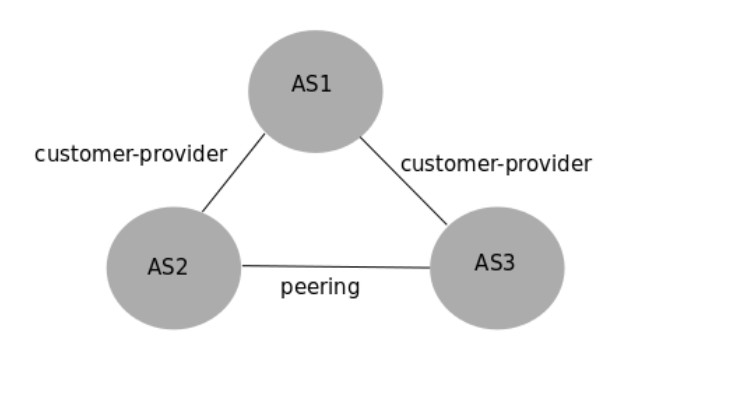
\includegraphics[width=120mm,height=80mm]{as}
		\label{as}
		\caption{Exemple}
	\end{figure} 
	
\section{Problèmes}
Nous n'avons pas de solution pour les 3 domaines possédant 2 préfixes, seulement le premier préfixe a été utilisé. Certains hôtes sont injoignables à partir de certains routeurs, nous n'avons pas réussi à trouver d'où cela pouvait provenir. 

\section{Conclusion}
Ce projet nous a permis de mieux comprendre certains principes de BGP ainsi que nous apprendre quelque base dans la modélisation d'une interconnexion de réseau.



\end{document}